\documentclass[conference]{IEEEtran}


\usepackage{cite}
\usepackage{pslatex} % -- times instead of computer modern, especially for the plain article class
\usepackage[colorlinks=false,bookmarks=false]{hyperref}
\usepackage{booktabs}
\usepackage{graphicx}
\usepackage{xcolor}
\usepackage{multirow}
\usepackage{comment}
\usepackage{listings}
%\usepackage{flushend} % even out the last page, but use only at the end when there is a bibliography
%\usepackage{minted}		% For inserting code
%\setminted[systemverilog]{
%	tabsize=3
%}
%\setminted[C]{
%	tabsize=3,
%	breaklines
%}
%\setminted[scala]{
%	tabsize=3,
%	breaklines
%}
\usepackage{xspace}		% For using \SV with trailing spaces
\usepackage{cleveref}	% Needed for correctly referencing listings
\usepackage{subfig}

\newcommand{\code}[1]{{\small{\texttt{#1}}}}
\newcommand{\SV}{SystemVerilog\xspace}


% fatter TT font
\renewcommand*\ttdefault{txtt}
% another TT, suggested by Alex
% \usepackage{inconsolata}
% \usepackage[T1]{fontenc} % needed as well?

%\newcommand{\todo}[1]{{\emph{TODO: #1}}}
\newcommand{\todo}[1]{{\color{olive} TODO: #1}}
\newcommand{\martin}[1]{{\color{blue} Martin: #1}}
\newcommand{\simon}[1]{{\color{green} Simon: #1}}
\newcommand{\abcdef}[1]{{\color{red} Author2: #1}}
\newcommand{\rewrite}[1]{{\color{red} rewrite: #1}}
\newcommand{\ducky}[1]{{\color{orange} Richard: #1}}
\newcommand{\kasper}[1]{{\color{purple} Kasper: #1}}
\newcommand{\hjd}[1]{{\color{pink} Hans: #1}}

% uncomment following for final submission
\renewcommand{\todo}[1]{}
\renewcommand{\martin}[1]{}
\renewcommand{\simon}[1]{}
\renewcommand{\kasper}[1]{}
\renewcommand{\ducky}[1]{}



%%% ZF
\usepackage{listings}
\lstset{
	columns=fullflexible,
	%        basicstyle=\ttfamily\footnotesize,
	basicstyle=\ttfamily\small,      
	%columns=fullflexible, keepspaces=true,
	numbers=left,    
	numberblanklines=false,
	captionpos=b,
	%	breaklines=true,
	escapeinside={@}{@},
	numbersep=5pt,
	language=C,
	tabsize=2,
	breakatwhitespace=true,
	breaklines=true,
	deletekeywords={for},
	%        keywordstyle=\ttfamily
	numbersep=5pt,
	xleftmargin=.10in,
	%xrightmargin=.25in
}

\newcommand{\longlist}[3]{{\lstinputlisting[float, caption={#2}, label={#3}, frame=tb, captionpos=b]{#1}}}

\title{ChiselVerify: An Open-Source Hardware Verification Library for
Chisel and Scala}

\author{
\IEEEauthorblockN{No Author Given}
\IEEEauthorblockA{No Institute Given}
}

%\author{\IEEEauthorblockN{Andrew Dobis, Tjark Petersen, Kasper Juul Hesse Rasmussen, Enrico Tolotto, \\
%Hans Jakob Damsgaard, Simon Thye Andersen, Richard Lin, Martin Schoeberl}\\
%\IEEEauthorblockA{\textit{Department of Applied Mathematics and Computer Science} \\
%\textit{Technical University of Denmark}\\
%Lyngby, Denmark \\\\
%\textit{Department of Electrical Engineering and Computer Sciences} \\
%\textit{UC Berkeley}\\
%Berkeley, CA \\\\
%andrew.dobis@alumni.epfl.ch, s186083@student.dtu.dk, s183735@student.dtu.dk, s190057@student.dtu.dk, \\
%s163915@student.dtu.dk, simon.thye@gmail.com, richard.lin@berkeley.edu, masca@dtu.dk}
%}


\begin{document}

\maketitle
\thispagestyle{plain}
\pagestyle{plain}


\begin{abstract}
Performance increase with general-purpose processors has come to a halt.
We can no longer depend on Moore's Law to increase computing performance.
The only way to achieve higher performance or lower energy consumption
is by building domain-specific hardware accelerators.
To efficiently design and verify those domain-specific accelerators, we need
agile hardware development. One of the main obstacles when proposing such a modern method
is the lack of modern tools to attack it. To verify a design in such a time-constrained development
method, one needs to have efficient tools both for design and verification.

This paper thus proposes ChiselVerify, an open-source library for verifying
circuits described in Chisel. It builds on top of the Chisel
hardware construction language and uses Scala to drive the verification process.
ChiselVerify increases the productivity of the verification engineer by allowing hardware testing to be done in a modern high-level programming environment.
The solution is well integrated into the existing Chisel universe, making it an extension of currently existing testing libraries.


%We implement ChiselVerify in a way inspired by the functionalities found in SystemVerilog. This allows one to use
%functional coverage, constrained-random verification, bus functional models, transaction-level modelling and much more
%during the verification process of a design in a contemporary high-level programming ecosystem.
\end{abstract}

\begin{IEEEkeywords}
digital design, verification, Chisel, Scala
\end{IEEEkeywords}

%\section{TODO}

%\begin{itemize}
%\item incorporate the reviews
%\item add \url{http://people.eecs.berkeley.edu/~ksen/papers/rfuzz.pdf} to related work
%\item Find a new venue abstract May 28: \url{http://www.iccd-conf.com/Home.html|} // Abstract due 11.06.21
%\item \hjd{Perhaps the use case is a bit too lengthy... Implementation details are not interesting here; the testing is, and it takes up little of the section.}
%\end{itemize}


%\begin{verbatim}
%Dear Martin Schoeberl:
%
%I am sorry to inform you that the following submission was not selected by the program committee to appear at SAMOS XXI 2021:
%
%ChiselVerify: An Open-Source Verification Method with Chisel and Scala
%
%The selection process was very competitive. Due to time and space limitations, we could only choose a small number of the submitted papers to appear on the program. Nonetheless, I still hope you can attend the conference.
%
%I have enclosed the reviewer comments for your perusal.
%
%Best Regards, 
%Matthias Jung, PC SAMOS XXI
%
%============================================================================ 
%SAMOS XXI 2021 Reviews for Submission \#33
%============================================================================ 
%
%Title: ChiselVerify: An Open-Source Verification Method with Chisel and Scala
%Authors: Andrew Dobis, Tjark Petersen, Kasper Hesse, Enrico Tolotto, Hans Damsgaard, Simon Andersen, Richard Lin and Martin Schoeberl
%
%
%============================================================================
%                            REVIEWER \#1
%============================================================================
%
%---------------------------------------------------------------------------
%Reviewer's Scores
%---------------------------------------------------------------------------
%Evaluation of the work and contributions (1-5): 3
%           Originality and Novelty (1-4): 3
%                         Relevance (1-5): 5
%            Overall Recommendation (1-4): 2
%                        Best Paper Award: No
%                  Your Familiarity (1-3): 3
%
%Detailed Comments
%---------------------------------------------------------------------------
%The paper presents ChiselVerify, an open source framework for verification of circuits modeled in Chisel. Chisel is a framework developed previously in other works. ChiselVerify appears to be based on ChiselTest, a previously developed testing framework for Chisel. ChiselVerify appears to extend ChiselTest with constraint based coverage.
%
%The paper definitely presents a valid contribution and ChiselVerify should be a very useful verification environment for Chisel. Unfortunately, the paper is badly written, with little structure to help the reader understand the contributions and navigate the different sections. Even basic questions, such as what exactly is ChiselVerify? what inputs does it take? what outputs does it produce? how is it implemented? what other software does it use? etc. are left untouched.
%
%As it stands, the paper reads more like a juxtaposition of different sections written by various people, with no connection to one another. I believe that a significant rewrite is necessary before publication.
%
%Ira. D. Baxter -> Ira D. Baxter
%---------------------------------------------------------------------------
%
%
%
%============================================================================
%                            REVIEWER \#2
%============================================================================
%
%---------------------------------------------------------------------------
%Reviewer's Scores
%---------------------------------------------------------------------------
%Evaluation of the work and contributions (1-5): 3
%           Originality and Novelty (1-4): 2
%                         Relevance (1-5): 3
%            Overall Recommendation (1-4): 2
%                        Best Paper Award: No
%                  Your Familiarity (1-3): 3
%
%Detailed Comments
%---------------------------------------------------------------------------
%This paper proposes ChiselVerify, an open-source tool for verifying circuits described in Chisel. The idea is both good and timely. However, I could not get a clear picture of what is ChiselVerify, and what are its strengths and weaknesses. Does it support testing FSMs? Possibly as the test example shows some, but how? This paper is an extension of [15]. How does it differ from that work? The authors claim the main contribution of this paper is ChiselVerify, an open-source verification library for hardware designs. As such I would expect the paper to focus on the description of the tool and its functionality.
%
%A section named "Verification of AXI4 Interfaced Components" is offered, and mentions "bus functional models" (BFMs). However it is unclear if any BFM is supported and what is the required effort to produce/include them
%
%Treadle: cite this work. This section appears interesting but it not a contribution of this paper
%
%A sorting hardware use case is described, but actual testing text consists of two parahgraphs 
%
%Overall which ether topic is interesting, the presentation lacks focus.
%---------------------------------------------------------------------------
%
%
%
%============================================================================
%                            REVIEWER \#3
%============================================================================
%
%---------------------------------------------------------------------------
%Reviewer's Scores
%---------------------------------------------------------------------------
%Evaluation of the work and contributions (1-5): 4
%           Originality and Novelty (1-4): 3
%                         Relevance (1-5): 4
%            Overall Recommendation (1-4): 3
%                        Best Paper Award: No
%                  Your Familiarity (1-3): 2
%
%Detailed Comments
%---------------------------------------------------------------------------
%This paper presents ChiselVerify, an open-source tool for verifying circuits described in Chisel. It builds on top of the Chisel language and uses Scala to drive the verification process, thus the effectiveness (productivity) of verification phases can be improved. 
%In general, the paper is easy to read and follow. The fact that the author released it as open source is well received. 
%The paper is useful to verification engineers.
%---------------------------------------------------------------------------
%
%
%
%============================================================================
%                            REVIEWER \#4
%============================================================================
%
%---------------------------------------------------------------------------
%Reviewer's Scores
%---------------------------------------------------------------------------
%Evaluation of the work and contributions (1-5): 4
%           Originality and Novelty (1-4): 2
%                         Relevance (1-5): 4
%            Overall Recommendation (1-4): 3
%                        Best Paper Award: No
%                  Your Familiarity (1-3): 2
%
%Detailed Comments
%---------------------------------------------------------------------------
%In this work, ChiselVerify, an open-source tool for verifying circuits described in Chisel, is proposed.It builds on top of the Chisel hardware construction language and uses Scala to drive the verification process.
%The manuscript is very well organized and written presenting thoroughly all the steps of the research. The target problem and its importance are presented and discussed in detail as well as the previous work. Also, the proposed design methodology are presented in a clear and detailed way. All the sections of the paper balance very effectively between the background information of each topic and the explanation of each implementation. Moreover, both the examples throughout the sections and the final example, it seems the ideal way to make a reader have a deep understanding of this work. Finally the fact that this work is in open source, underlines and emphasizes the reliability of this work. 
%However an interesting information would be a comparison of this kind of verification(that this work proposes) compared to more conservatives methods in relation to time needed for each method, and effectiveness.
%---------------------------------------------------------------------------
%
%
%-- 
%SAMOS XXI 2021 - https://www.softconf.com/l/samos-xxi
%\end{verbatim}


\section{Introduction}
\label{sec:introduction}

We can no longer depend on Moore's Law to increase computing performance~\cite{dark-silicon:2011}.
Performance increase with general-purpose processors has come to a halt.
The only way to achieve higher performance or lower energy consumption
is by building domain-specific hardware accelerators~\cite{domain-hw-acc:2020}.
These accelerators can be built as chips or in FPGAs in the cloud.
%The production of a chip is costly. Therefore, it is essential to get
%the design right at the first tape-out. Thorough testing and verification of the design is mandatory.

To efficiently develop and verify those accelerators, we can learn from software development trends such as agile software development~\cite{agile:manifesto}.
We believe that we need to adapt to agile hardware development~\cite{henn-patt:turing:2019}.

Furthermore, as accelerators become part of the cloud service, i.e., FPGAs in the cloud,
software developers will increasingly need to adapt critical algorithms to FPGAs to enhance performance.
Hence, it is imperative to make accelerator design accessible for software developers.
By adapting hardware accelerator design to the methods and tools of contemporary software design,
it is possible to bridge both domains catering to a more uniform hardware/software development process.

A few years ago, the two main design languages, Verilog and VHDL, dominated the
design and testing of digital circuits.
%However, both languages are decades behind
%modern languages for software development.
However, compared to software development and testing, digital design and testing methods/tools 
lack several decades of development.
We thus developed a method and concrete tools for agile hardware development.
ChiselVerify combines tools, languages, development, and testing methods from the last decades in
software development and applies them to hardware design.

Therefore, we aim to raise the tooling level for a digital design to increase productivity.
ChiselVerify is based in the hardware construction language Chisel~\cite{chisel:dac2012},
which itself is embedded in Scala.


%Using the power and flexibility of Chisel Blackboxes, our tool can be used to verify
%designs implemented in any of the major hardware description languages (i.e., VHDL or Verilog)
%with little overhead. Furthermore, golden models described in any programming language can be
%used using the Java JNI. Our work builds upon existing open-source projects and 
%is thus also open-source.

We developed a verification framework in Scala.
This framework is inspired by the Universal Verification Method (UVM) but leverages Scala's conciseness with the
combination of object-oriented and functional programming.
An initial experiment of testing the accumulator circuit of the Leros processor~\cite{leros:arcs2019}
showed that a test written with UVM was about 800 lines of code, where a Scala-based
test was around 80 lines of code~\cite{verify:chisel:2020}.
However, UVM supports more functionalities than a plain ChiselTest~\cite{chisel:tester2} in Scala.

%Within our verification framework, we support mixed language verification.
%Verilog can easily be combined with Chisel, as Chisel generates Verilog, and
%we use ChiselTest as a driver for the open-source Verilog simulator Verlator.
%With Yosys synthesis suite~\cite{Yosys} and GHDL~\cite{ghdl}
%we can translate VHDL into Verilog.
%
%A verification method is only usable when it can handle mixed-source designs.
%This means a Scala driven method must be able to test components written in Verilog,
%VHDL, and SystemVerilog.
%
%Chisel has support for black boxes, which allows the use of Verilog code within the Chisel design.
%Therefore, it is relatively easy to integrate Verilog components when wrapped into a black box.
%However, this forces Chisel to use Verilator instead of Treadle to run the simulation, impacting
%startup time.
%
%Chisel does not fully support VHDL. It can support VHDL using VCS, but there is no
%open-source solution available for VHDL simulation. For companies with a lot of source code written in VHDL this is a concern, as they must be able to integrate their existing IP in a Scala/Chisel based design and verification workflow.
%All major commercial simulation and synthesis tools support mixed-language designs, but no open-source tools exist that provide the same functionality.


The main contribution of this paper is ChiselVerify~\footnote{https://github.com/chiselverify/chiselverify}, an open-source verification library for hardware designs.

The paper is organized into 6 sections.
Section 2 describes related work.
Section 3 describes background on hardware verification.
Section 4 describes our solution for enabling verification in Chisel, namely ChiselVerify.
Section 5 explores ChiselVerify on an industry-provided use case.
Section 6 concludes.

\section{Related Work}
%\todo{\url{https://capra.cs.cornell.edu/latte21/}}

SystemVerilog is an extension of Verilog. Many non-synthesizable extensions are intended
to write more advanced test benches. SystemVerilog adds object-oriented programming
for those test benches. However, in contrast to Chisel, the object-oriented addition cannot be
used for hardware description.
SystemVerilog contains certain constructs capable of gathering coverage information~\cite{spear2008systemverilog}, such as statement and functional coverage, in a manner similar to what we have developed. SystemVerilog can thus be used, along with the generated Verilog code, for the verification of a Chisel design. However, this is much more cumbersome than the purely Scala-based workflow that our solution offers. When it comes to functional coverage, our solution offers several features that SystemVerilog does not. For example more interesting \texttt{CoverPoints} that can take temporal relations into account and generalized functional bins that work using purely user-defined hit conditions, whilst SystemVerilog only offers bins that cover value ranges or transitions. These more advanced features are possible thanks to the functional nature of Scala. 

The \textit{Universal Verification Methodology} (UVM) was created as a standardized way of writing test benches on top of SystemVerilog. It allows for the creation of reusable test-benches (i.e., using the same test for multiple designs)~\cite{uvm2015}. However, it is verbose, and even a simple test requires around 1000 lines of SystemVerilog code. UVM thus requires a decent initial time-investment but is reusable once it gets up and running. This method can be used to verify Chisel designs, however the fact that UVM's methods differ so much from more traditional test benches, makes it less accessible than the simpler approach done by ChiselTest.


Other projects have also focused on applying software testing techniques to hardware verification. RFuzz~\cite{rfuzz2018} focuses on creating a generalized method that enables efficient ``coverage-guided fuzz mutational testing''. This method relies on FPGA-accelerated simulation and new solutions allowing for quick and deterministic memory resetting, to efficiently use fuzzing (i.e. randomized testing, where the random seeds are updated depending on certain coverage results) on RTL circuits. The coverage metrics used in this solution are automated and based on branch coverage. This work offers a different type of solution. While we work mostly on verification functionalities inside a language, RFuzz delivers an efficient way to use said functionalities in order to ameliorate testing. RFuzz uses functional coverage tools in order to guide its randomized testing. A similar result could be obtained by combining the Constrained Random Verification and Functional Coverage tools that are available in ChiselVerify.

\texttt{Chisel3.formal}  is a formal verification package containing a set of tools and helpers for formally verifying Chisel modules~\cite{chisel:formal}. The approach taken here is quite different from what we have developed. Rather than creating a set of tools that supplement the current chisel testing pipeline, \texttt{chisel3.formal} rather proposes a different way of testing, based around defining a set of formal checks that a design must pass in order to be considered as functional. These checks can, for example, look like: \texttt{past(io.out, 1) (pastIoOut => \{ assert(io.out >= pastIoOut) \})} which guarantees that the current module will never decrease its output from one cycle to the next. These formal checks can then be verified by calling the \texttt{verify(module)} function. 

This approach is similar to software contracts in Scala. The main difference between our solution and this one is that here the rules are written on a per-module basis and are thus directly linked to the Chisel code, while our solution rather focuses on checking that a suite of test-benches are testing the right things. The \texttt{chisel3.formal} package has also been extended in \texttt{kiwi-formal}~\cite{chisel:kiwi-formal} and \texttt{dank-formal}~\cite{chisel:dank-formal}, leading to multiple different versions of it, each adding their own additional formal rule templates. 

As far as we know, ChiselVerify is the only verification framework allowing for the easy use of verification functionalities, well integrated into the ChiselTest-Chisel ecosystem.

\section{Background}
\label{sec:background}

This section presents a brief overview of what hardware verification is. We will also talk about Chisel and the current solutions that exist in it with regards to the verification of digital designs.

\subsection{Verification of Digital Designs}
Verification of digital designs refers to the testing of a design before it has been taped-out~\cite{spear2008systemverilog}. This is in contrast to validation, which refers to testing a taped out version of a digital circuit. 
SystemVerilog~\cite{SystemVerilog} is one of the main languages used for verification.
This is due to the wide variety of verification-centric functionalities that the language offers, which focus on improving the efficiency of writing test-benches rather than the testing itself.
The language enables verification engineers to define constraint-driven randomized test-benches as well as define metrics to gather functional coverage data related to a test-suite. 
However, the verification functionalities are quite limited and being embedded in a low-level language makes writing tests quite complex. 
The three main verification features that we are interested in are: functional coverage, Constrained random verification, and bus functional models.

\subsubsection{Functional Coverage}
One of the main tools used in verification is test coverage. 
This allows verification engineers to measure their progress throughout the testing process and have an idea of how effective their tests actually are. 
Coverage can be separated into two distinct categories: code coverage and functional coverage. 
Code coverage defines a quantitative measure of the testing progress, \textit{``How many lines of code have been tested?''}, whereas functional coverage gives a rather qualitative measure, \textit{``Which functionalities have we tested?''}~\cite{spear2008systemverilog}.
Functional coverage allows one to have a way of measuring how correctly the specification has been implemented. Functional coverage is measured relative to a verification plan, which includes the three following components:

\begin{itemize}
  \item \texttt{Bin}s: Ranges of values that should be tested for (i.e., expected values of a given port).
  \item \texttt{CoverPoint}s: Ports that need to be sampled in the coverage report defined using a set of \texttt{Bin}s.
  \item \texttt{CoverGroup}s: Sets of \texttt{CoverPoint}s that need to be sampled at the same time.
\end{itemize}

A verification plan that includes these three components tells the coverage reporter which ports need to be sampled in order to generate a report.

\begin{figure*}
  \centering
    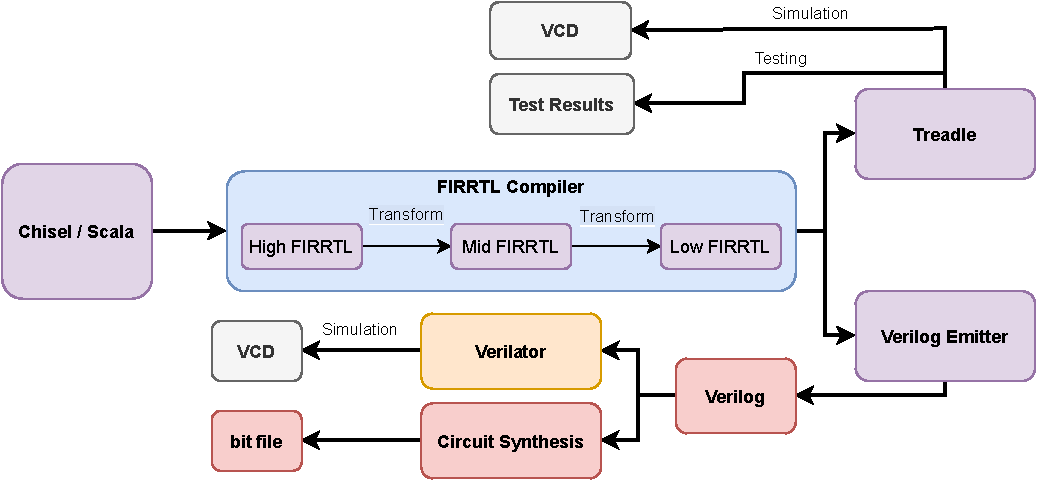
\includegraphics[width=0.8\linewidth]{Chisel_FIRRTL_VERILOG.pdf}
    \caption{Overview of the Chisel compilation pipeline.}
\label{fig:chisel-pipe}
\end{figure*}


\subsubsection{Constrained Random Verification}
As described earlier, the complexity of digital design is increasing with the capacity of the silicon. Traditionally, verification engineers would write a number of directed tests each focusing on one or more of a component's functionalities, but this approach becomes impractical for larger designs. Instead, a uniformly randomized verification methodology may be applied; constrained random verification, which is a combined effort of constraint programming and coverage-based methodologies.
Using constrained random inputs, a relatively small test suite can, statistically, cover many of a component's functionalities. 
The constraints help to ensure that no invalid input combinations that would not appear during regular operation are applied~\cite{MehtaCRV2018}.

With constraint programming, the user describes the problem in a declarative way. A subset of these problems is the so-called constraint satisfaction problems (CSP), which are mathematical problems defined as a set of objects whose state must satisfy several constraints. CSP represents the entities of a problem as a finite homogeneous collection of constraints. CSP solvers thus serve well as the basis for generating sets of constrained random signal values for verification.

SystemVerilog has native support for constrained random data types and a built-in CSP solver. Variables declared with the \texttt{rand} keyword are randomizable upon calling a \texttt{randomize} method.

\subsubsection{Bus Functional Models}
One solution to the ever-increasing complexity of digital designs often exploited by design engineers is to use standardized interfaces or buses of multiple signals. Doing so enables reuse and interchangeability of different implementations of the same component. Many synthesis tools, including Xilinx's Vivado, provide IP generators whose output IP blocks are equipped with such standard interfaces. Verification of components with such interfaces is most easily handled with so-called bus functional models (BFMs), which abstract reading and writing of signals to a transaction level. That is, using a BFM, a verification engineer can reduce several lines of code representing, e.g., a write transaction, to just a single call to a standardized method.


\subsection{Digital Design with Chisel}
Out verification library is used for designs described in Chisel.
Chisel is a ``Hardware Construction Language'' embedded in Scala, used to describe digital circuits~\cite{chisel:dac2012}.
This language is more high-level than the traditional hardware description languages, such as VHDL or Verilog, and allows for object-oriented and functional programming in the context of digital design.
One of the main aspects of Chisel that makes it so compelling is its full integration in the Java/Scala ecosystem.

Since Chisel and Scala are executing on the Java virtual machine (JVM), they have a very good interoperability with Java. 
We can therefore leverage a large pool of Java and Scala libraries for hardware design and verification. 
Furthermore, the packaging system in Scala/Java simplifies integration of external components.
Open source hardware components in Chisel can thus be organized in the same manner as software libraries in Maven servers.

Working in the JVM also allows for the use of the Java native interface, which enables JVM based languages to call C functions.
This enables co-simulations between Scala testers, Chisel designs, and a C-based golden model. 
This should allow companies to keep their existing C models, but move their simulation workflow into Scala/Chisel testers.

Chisel is solely a hardware \emph{construction} language, and thus all valid Chisel code maps to synthesizable hardware.
By separating the hardware construction and hardware verification languages, it becomes impossible to write non-synthesizable hardware and, in turn, speeds up the design process.

Chisel translates the hardware description into an intermediate representation called FIRRTL~\cite{firrtl}. It then performs multiple optimization stages, called transforms, during which high-level concepts, such as a functional map or vectors, are compiled into lower level concepts that map onto what we normally see in a Verilog or VHDL description. Once that is done, the newly transformed FIRRTL, called Low FIRRTL, can be used either for simulation, using an execution engine such as Treadle, or for synthesis by translating it into Verilog which is then used to generate the synthesized circuit. Note that the final Verilog description may also be used for simulation purposes using engines such as Verilator~\cite{verilator}. Figure~\ref{fig:chisel-pipe} shows an overview of the Chisel compilation pipeline.


\subsection{Testing Chisel Designs}
A digital design described in Chisel can be tested with ChiselTest~\cite{chisel:tester2}, a non-synthesizable testing framework for Chisel.
ChiselTest emphasizes on usability and simplicity while providing ways to scale up in complexity.
Fundamentally, ChiselTest is a Scala library that provides access into the simulator through
operations like poke (write value into circuit), peek (read value from circuit), and step (advance time).
As such, tests written in ChiselTest are just Scala programs, imperative code that runs one line after the next.
This structure uses the latest programming language developments that have been implemented into Scala
and provides a clean and concise interface.

Furthermore, ChiselTest tries to support best testing practices from software engineering.
Its lightweight syntax encourages writing targeted unit tests by making small tests easy.
A clear and clean test code also enables the test-as-documentation pattern,
demonstrating a module's behavior from a temporal perspective.

ChiselTest is missing fundamental verification functionalities that can improve the verification efficiency of Chisel designs. 
It is currently not possible to do things such as constrained random testing or obtaining functional coverage results while solely relying on the ChiselTest framework. 
Functionalities such as those are crucial when it comes to efficiently verifying one's design and this lack is probably one of the factors that is holding back some engineers thinking about switching to Chisel. 

\section{Verification with Chisel}

We propose ChiselVerify, a verification library based entirely in Scala. ChiselVerify uses the device under test (DUT) interfacing features from ChiselTest in order to enable three main verification functionalities in Chisel: functional coverage, constrained random verification, and bus functional modeling. We also show how our framework can be used to create a bus functional model, by creating one for the standardized AXI4 interface. The following subsections explain each functionalitie and present how to use it.

\subsection{Coverage in Chisel}


In our solution, we give the verification engineer access to new constructs allowing the definition of a verification plan and the creation of a functional coverage report directly integrated into the Chisel testing framework.

%\subsubsection{Code Coverage with Treadle}  
%The first part of our solution is about code coverage, more specifically line coverage that was added to the Treadle FIRRTL execution engine. Treadle is a common FIRRTL execution engine used to simulate designs implemented in Chisel. This engine runs on the FIRRTL intermediate representation code generated by a given Chisel implementation and allows one to run user-defined tests on the design using frameworks like \textit{iotesters} or the more recent \textit{ChiselTest}. In our pursuit of creating a verification framework, we found that one way to obtain line coverage would be to have our framework run on an extended version of Treadle that was capable of keeping track of said information.
%
%The solution that was used to implement line coverage was based off of a method presented by Ira. D. Baxter~\cite{branch-cov-made-easy:2002}. The idea is to add additional outputs for each multiplexer in the design. These new ports, which we will call \textit{Coverage Validators}, are set depending on the paths taken by each multiplexer and that information is then gathered at the end of each test and maintained throughout a test suite. Once the testing is done, we used the outputs gathered from the \textit{Coverage Validators} to check whether or not a certain multiplexer path was taken during the test, all of this resulting in a branch coverage percentage \hjd{Should this be line coverage?}.
%
%This was implemented in Treadle by creating a custom pass of the FIRRTL compiler that traverses the Abstract Syntax Tree (\textit{AST}) and adds the wanted outputs and coverage expressions into the source tree. Once that is done, the \texttt{TreadleTester} samples those additional outputs every time the \texttt{expect} method is called and keeps track of their values throughout a test suite. Finally it generates a Scala \texttt{case class} containing the following coverage information:
%
%\begin{itemize}
%  \item The multiplexer path coverage percentage.
%  \item The coverage Validator lines that were covered by a test.
%  \item The modified LoFIRRTL source code in the form of a \texttt{List[String]}.
%\end{itemize}
%
%The \texttt{CoverageReport} case class can then be serialized, giving, e.g., the following report:
%\begin{verbatim}
%COVERAGE: 50.0% of multiplexer paths tested
%COVERAGE REPORT:
%
%+ circuit Test_1 :
%+   module Test_1 :
%+     input io_a : UInt<1>
%+     input io_b_0 : UInt<2>
%+     input io_b_1 : UInt<2>
%+     input clock : Clock
%+     output io_cov_valid_0 : UInt<1>
%+     output io_cov_valid_1 : UInt<1>
%+     output out : UInt<2>
%+   
%+     io_cov_valid_0 <= io_a
%-     io_cov_valid_1 <= not(io_a)
%+     out <= mux(io_a, io_b_0, io_b_1)
%\end{verbatim}
%The example above is taken for a simple test, where we are only testing the path where \texttt{in\_a} is 1. This means that, since we only have a single multiplexer, only half of our branches have been tested and we would thus want to add a test for the case where \texttt{in\_a} is 0. The report can thus be interpreted as follows:
%
%\begin{itemize}
%  \item "\texttt{+}" before a line means that it was executed in at least one of the tests in the test suite.
%  \item "\texttt{-}" before a line means that it wasn't executed in any of the tests in the test suite.
%\end{itemize}
%
%Treadle thus allows us to obtain coverage at the FIRRTL level. A more interesting result would be if the FIRRTL line coverage would be mapped to the original Chisel source. This is possible but challenging, since Treadle only has access to the original source code through \textit{Source locators} which map some of the FIRRTL lines back to Chisel. This means that the code can only be partially mapped and the remainder will have to be reconstructed using some smart guessing.

In order to implement the different components needed for functional coverage in Scala, we needed to be able to do the following:

\begin{itemize}
  \item Define a verification plan (using constructs similar to \texttt{CoverPoint} and \texttt{Bin}).
  \item Sample DUT ports (for example by hooking into the ChiselTest framework).
  \item Keep track of bins to sampled value matches (using a database).
  \item Compile all of the results into a comprehensible coverage report.
\end{itemize}

Implementing these elements was done using a structure based around a top-level element known as the \texttt{CoverageReporter}, which allows the verification engineer to define a verification plan using a \texttt{register} method. The \texttt{register} method stores \texttt{CoverPoint} to \texttt{Bin} mappings inside a \texttt{CoverageDB} (DB being short for database) object. Once the verification plan is defined, ports may be sampled using the \texttt{sample} method, which is implemented based on ChiselTest peeking capabilities. At the end of a test suite, a functional coverage report can be generated using the \texttt{printReport} method, which summarizes the results stored in the database.\\\\

\begin{lstlisting}[language=scala]
val cr = new CoverageReporter
cr.register( // Declare CoverPoints
  CoverPoint(dut.io.accu, "accu", // CoverPoint 1
    Bins("lo10", 0 to 9) ::
    Bins("First100", 0 to 99) ::
    Nil) ::
  CoverPoint(dut.io.test, "test", // CoverPoint 2
    Bins("testLo10", 0 to 9) ::
    Nil) ::
  Nil,
  // Declare cross points
  Cross("accuAndTest", "accu", "test", 
    CrossBin("both1", 1 to 1, 1 to 1) ::
    Nil)::
  Nil
)
\end{lstlisting}

The above code snippet is an example of how to define a verification plan using our coverage framework. One concept, that is used in the example verification plan, is the idea of \textit{cross coverage} defined using the \texttt{Cross} construct. Cross coverage allows one to specify coverage relations between \texttt{CoverPoint}s. This means that a cross defined between, e.g., \texttt{CoverPoint} $a$ and \texttt{CoverPoint} $b$ will be used to gather information about when $a$ and $b$ have certain values simultaneously~\cite{spear2008systemverilog}.
Thus, in our example verification plan, we are checking that \texttt{accu} and \texttt{test} take the value 1 at the same time.

Once our verification plan is defined, we need to decide when we want to sample our cover points. This means that at some point in our test, we have to tell our \texttt{CoverageReporter} to sample the values of all of the points defined in our verification plan. This can be done, in our example, simply by calling \texttt{cr.sample()} when we are ready to sample our points. Finally once our tests are done, we can ask for a coverage report by calling \texttt{cr.printReport()} which results in the following coverage report: \\\\
\begin{verbatim}
=============== COVERAGE REPORT ===============
================= GROUP ID: 1 =================
COVER_POINT PORT NAME: accu
BIN lo10 COVERING 0 to 9 HAS 8 HIT(S) = 80%
BIN First100 COVERING 0 to 99 HAS 9 HIT(S) = 9%
===============================================
COVER_POINT PORT NAME: test
BIN testLo10 COVERING 0 to 9 HAS 8 HIT(S) = 80%
===============================================
CROSS_POINT accuAndTest FOR POINTS accu AND test
BIN both1 COVERING 1 to 1 CROSS 1 to 1 HAS
1 HIT(S) = 100%
===============================================
\end{verbatim}
In the above report, we can see that our two \texttt{CoverPoint}s are listed and that each one of their \texttt{Bins} has an associated number of hits. This represents how many times the port had a unique value within the given range. A coverage percentage is then given for each bin, representing the ratio between the number of hits and the total number of possible values in the range.
The current coverage results can also be used to implement a more advanced automated constraint modification flow by simply using the \texttt{binNcases} method of the \texttt{CoverageReport} case class returned by the coverage reporter. 

Another element that our framework offers, is the possibility to gather delayed coverage relationships between two coverage points. The idea is similar to how a \texttt{Cross} works, but this time rather than sampling both points in the same cycle, we rather look at the relation between one point at the starting cycle and another point sampled a given number of cycles later. This number of cycles is called the \texttt{delay} and there are currently three different ways to specify it:  
\begin{itemize}
  \item \texttt{Exactly} delay, means that a hit will only be considered if the second point is sampled in its range a given number of cycles after the first point was.
  \item \texttt{Eventually} delay, means that a hit will be considered if the second point is sampled in its range at any point within the following given number of cycles after the first point was.  
  \item \texttt{Always} delay, means that a hit will be considered if the second point is sampled in its range during every cycle for a given number of cycles after the first point was sampled.
\end{itemize}

Finally, we exploit the functional nature of Scala in order to allow for conditional cover points, which offer the possibility to create fully custom hit-consideration rules using a user-defined condition. 
This allows the user to check for arbitrary relations between an arbitrary number of ports rather than having to rely solely on value ranges. 
One could then, e.g. create a bin that considers a hit every time all fields in a vector are equal. 
This is only possible thanks to higher-order functions. 
These can be defined in two different ways. 
A first way is to use regular \texttt{CoverPoint}s and add a \texttt{Condition} argument to the bin that would want them. 
This would mean that the condition would filter out values that can be considered for a hit in the given range and can only be applied to a single port. 
An other way would be to use a \texttt{CoverCondition}, which is similar to a \texttt{CoverPoint}, but can be applied to an arbitrary amount of ports and only uses \texttt{Condition}s when considering a hit.
The report shows the number of hits that each condition had throughout the test suite.
The user also has the choice of adding an ``expected number of hits'' to each condition.
This allows for a final percentage to be shown along side the number of hits.
%Another method to compute a coverage percentage would be to create the set of every possible value combination between the given ports, then filtering them out using the condition and getting the size of the remaining possible values.
%This, however, requires an expensive Cartesian product to be computed, which results in a complexity of $O(w^{p})$, where $w$ is the maximum port width and $p$ is the number of ports.
%This method is thus unusable any real-world applications, which is why we opted for the first one.

All of these features allow for the definition of complex verification plans that can be used to represent any given specification, making it possible to verify the correct testing of any design.
Supporting a coverage measure directly in the testing tool also enables modern verification strategies such as constrained random verification.

\subsection{Constrained Random Verification}

\martin{We never mention that we are using someone elses solver. This is on
the boarder to cheating.}

%\begin{lstlisting}[caption={Random object in SystemVerilog}, label={lst:randobjsysv}]
%typedef enum {UNICAST=11,MULTICAST,BROADCAST} pkt_type;
%
%class frame_t;
%    rand pkt_type ptype;
%    rand integer len;
%    rand bit  [7:0] payload [];
%    constraint common {
%        payload.size() == len;
%    }
%    // Constraint the members
%    constraint unicast {
%        len <= 2;
%        ptype == UNICAST;
%    }
%    // Constraint the members
%    constraint multicast {
%        len >= 3;
%        len <= 4;
%        ptype == MULTICAST;
%    }
%endclass
%\end{lstlisting}

%Listing \ref{lst:randobjsysv} shows a class named \code{frame\_t} in SystemVerilog. It uses the \code{rand} keyword for variables \code{len}, \code{ptype}, and \code{payload}.
%Therefore these are the variables that can be randomized. Then constraints to these variables are applied and declared by the \code{common},  \code{unicast},
%and \code{multicast} constraint groups. Each class in SystemVerilog has an intrinsic method called \code{randomize()}, which causes new values to be selected
%for all the variables declared with the rand keyword. The selected value for each variable will respect the constraints applied to it. If there are
%\code{rand} variables that are unconstrained, a random value inside their domain will be assigned. Combining random classes using the inheritance OOP
%paradigm allows the creation of general-purpose models that can be constrained to perform domain-specific functions. 

SystemVerilog serves as an inspiration for our work, but we diverge from SystemVerilog by exploiting the functional nature of Scala. We have implemented a CSP solver in Scala based on the method described in~\cite{russell2002artificial}. The implementation is composed of two main components. The first one is the CSP solver itself, which uses a combination of backtracking and arc consistency to generate solutions for well-defined problems. The second component is a domain specific language, which allows users to declare and randomize objects.

\subsubsection{Constraint Programming with ChiselVerify}
In order to begin writing constrained random objects using our library, one must define a \texttt{class} which extends the \texttt{RandObj} trait while initializing it with a \texttt{Model}. A \texttt{Model} represents a database in which all of the \texttt{RandObj}'s random variables and constraints are stored. This \texttt{RandObj} will then contain all of the constraints and random variables that we will use in our constrained random tests. There are two main constructs that can be defined inside of a \texttt{RandObj}: random variables and constraints.

\paragraph{Random variables} There are two main types of random variables that can be defined inside of a \texttt{RandObj}: \texttt{Rand} and \texttt{Randc}. Both types are declared using a lower and an upper bound. \texttt{Rand} random variables  are regular uniformly distributed values found between the given upper and lower bounds. \texttt{Randc}, however, represents a Random-cyclic variable, meaning that the values found between the lower and upper bound will not be repeated until all of the values have been covered. For example, if we create a \texttt{Randc(0, 5)}, we will never get the same value twice if we sample it 6 times, however on the 7th sampling the cycle will be reset and we will start to re-obtain old values.

\paragraph{Constraints} Once all of the random variables have been declared, we can start declaring constraints for these variables. Constraints can either be defined alone or in \texttt{ConstraintGroup}s. Constraint operators are preceded by the \texttt{\#} symbol. These constraints can be on a single random variable or an on expression containing multiple variables, like for example a constraint can contain the subtraction of two random variables. Conditional constraints may also be defined using the \texttt{IfCond} and \texttt{ElseC} constructs. All of these constraints can then be enabled and disabled when needed throughout the test suite.

\paragraph{Using a RandObj} When we defined our random variables and their constraints, we can use them in our tests. We instantiate the previously defined \texttt{RandObj} and then randomize it using the \texttt{randomize} method which returns \texttt{true} if the constraints were able to be solved by the CSP solver. The random variables can then be accessed using their respective \texttt{value()} methods. We will show how to use the constrained random verification tool with a simple example shown in Listing~\ref{lst:randobjscala}.

%As an example, consider listing~\ref{lst:randobjscala} which shows the declaration of a NoC packet (or frame) random bundle with four fields; the packet type \texttt{pType}, the packet length \texttt{len}, whether the packet will be repeated \texttt{noRepeat}, and the packet payload \texttt{payload}. The packet type takes one of three possible values declared in a separate enumeration object \texttt{pktType}. Constraints are declared as \texttt{constraintBlock}s including one or more unary or binary constraints, which are functions operating on the random fields. In this case, different constraints apply to the \texttt{len} field depending on the packet type field \texttt{pType}.

\begin{lstlisting}[language=scala, caption={Usage of a random object.}, label={lst:randobjscala}]    
class Packet extends RandObj(new Model(3)) {
    val idx = new Randc("idx", 0, 10)
    val size = new Rand("size", 1, 100)
    val len = new Rand("len", 1, 100)
    val payload: Array[Rand] = Array.tabulate(11)(
        new Rand(s"byte[$_]", 1, 100)
    )

    //Example Constraint with operations
    val single = payload(0) #= (len #- size)
	
    //Example conditional constraint
    val conditional = IfCon(len #= 1) {
        payload.size #= 3
    } ElseC {
        payload.size #= 10
    }
    val idxConst = idx #< payload.size
}
//Instantiate RandObj
val pckt = new Packet

//Check that the constraints were solvable
assert(pckt.randomize)

// [...] ChiselTest boilerplate [...]

//Example use of random variables in a DUT
dut.portA.poke(
    pckt.payload(pckt.idx.value()).value()
)

\end{lstlisting}

Listing~\ref{lst:randobjscala} shows how we can create a random object with a given seed. We also show that it is possible to have collections of random variables and create constraints on those collections. This is done in the \texttt{payload} random variable. We then also demonstrate the use of conditional constraints in the \texttt{conditional} random variable, where the constraint depends of the value of the \texttt{len} random variable. An other example could be to poke DUT ports in a loop that randomizes the \texttt{RandObj} at each iteration. This is just a basic example to show how our constraint-specific language can be used to write constrained random tests.

%Listing \ref{lst:randobjscala}, shows an example of a random object. To declare a random object, the user has to extend the class from the \code{Random} base-class provided by the library. After that, each random variable has to be declared of type \code{RandInt} and initialized with the \code{rand} macro. Finally, inheriting the Random base class exposes the method \code{random} which assigns random values to the random fields of the class.

Combining constraint random objects with the provided coverage features enables writing tests very efficiently. However, this may be further optimized by abstracting away groups of wires and operating on an operation or transaction level instead.

\subsection{Verification with Bus Functional Models}
In this work, we provide an example BFM for AXI4, an open standard by ARM~\cite{axi4standard}. The example works only for AXI4, but it can easily be extended to support other buses. Let us first give a brief introduction to AXI4.

\subsubsection{Introduction to AXI4}
The Advanced eXtensible Interface (AXI) protocol by ARM is a highly flexible interconnect standard based around five independent channels; three for write operations and two for read operations. Operations, known as transactions, consist of a number of transfers across either set of channels. All channels share a common clock and active-low reset and base their transfers on classic ready-valid handshaking. It is designed with memories in focus that supporte multiple outstanding transactions and out-of-order completion. The write channels are \textit{Write Address}, \textit{Write Data}, and \textit{Write Response}, as shown in Figure~\ref{fig:axi4w}. The read channels are \textit{Read Address} and \textit{Read Data} shown in Figure~\ref{fig:axi4r}.
% Ms does not understand what the simplification is
% shows how the different channels can be simplified into a write transaction and a read transaction.

\begin{figure*}[t]
  \centering
  \subfloat[Write channels.\label{fig:axi4w}]{
    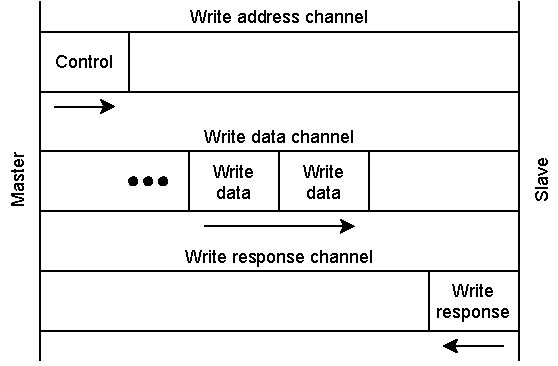
\includegraphics[width=0.45\linewidth]{WriteTrx.pdf}
  }
  \hfill
  \subfloat[Read channels.\label{fig:axi4r}]{
    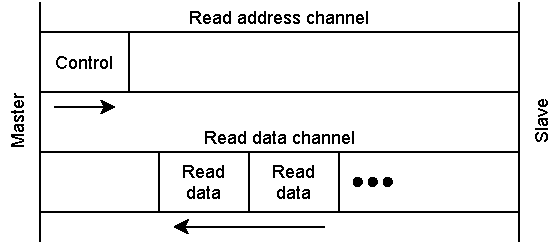
\includegraphics[width=0.45\linewidth]{ReadTrx.pdf}
  }
  \label{fig:axi4}
  \caption{An overview of the channels defined in the AXI4 standard.}
\end{figure*}

%\begin{itemize}
%  \item \textit{Write Address} for transferring transaction attributes from master to slave
%  \item \textit{Write Data} for transferring write data and strobe from master to slave
%  \item \textit{Write Response} for transferring transaction status of a writes from slave to master
%  \item \textit{Read Address} same as \textit{Write Address}, but for reads
%  \item \textit{Read Data} for transferring read data from slave to master
%\end{itemize}

\martin{Is it really specified that write address has to be sent before the data?
I guess those channels are independent.}
Consider for example a write transaction of 16 data elements. First, the master provides transaction attributes (e.g., target address and data size) as a single transfer over the \textit{Write Address} channel, then the master transfers the 16 data elements one at a time over the \textit{Write Data} channel, and finally, the slave indicates the status of the transaction over the \textit{Write Response} channel. The \textit{Read Address} and \textit{Read Data} channels may operate independently at the same time. A full description is available in \cite{axi4standard}.

\subsubsection{Implementation}
Our implementation of an AXI4 BFM includes bundles defining the five different channels, abstract classes representing both master and slave entities, transaction-related classes, and the BFM itself, the \texttt{FunctionalMaster} class. The BFM is parameterized with a DUT that extends a \texttt{Slave} class and provides a simple, transaction level interface to control the DUT. As such, its two most important public methods are \texttt{createWriteTrx} and \texttt{createReadTrx} which do exactly as their names indicate; create and enqueue write and read transactions.

Internally, the BFM makes use of ChiselTest's multithreading features to allow for (a) non-blocking calls to the aforementioned methods (i.e., one can enqueue multiple transactions without waiting for their completion) and (b) emulating the channel independence more closely. As such, when, for example, a write transaction is enqueued and no other write transactions are in-flight, the BFM spawns three new threads, one for each required channel. The threads each handle the handshaking necessary to operate the channels.

\subsubsection{A Test Example}
Consider as an example using the BFM to test a module called \texttt{Memory}, which is shown below. Creating a write transaction with 16 data elements (minimum burst length is 1, hence \texttt{len = 15} means a burst of 16 items) takes just one call to a method the majority of whose arguments have default values. It is equally simple to create a subsequent read transaction. Beware that due to channel independence, not waiting for a write to complete before starting to read from the same address may return incorrect results depending on the implementation of the DUT.
\begin{lstlisting}[language=scala, caption={Using the AXI4 BFM with ChiselTest}, label={lst:axitest}]
class MemoryTester extends FlatSpec with ChiselScalatestTester {
  behavior of "My Memory module"
  it should "write and read" in {
    test(new Memory()) { dut =>
      val bfm = new FunctionalMaster(dut)
      master.createWriteTrx(0, Seq.fill(16)(0x7FFFFFFF), len = 15, size = 2)
      master.createReadTrx(0, len = 15, size = 2)
    }
  }
}
\end{lstlisting}

\section{Use Case: Sorting in Hardware}

In the process of our research we received a use case from Microchip, in the form of a specification.
We implemented and used it to evaluate our verification library.

\subsection{Specification}

The provided use case is a hardware implementation of a priority queue. It can be used in real-time systems where scheduling capabilities are required. For instance, time stamps for deadlines can be inserted and sorted, such that the host system has access to the closest deadline.

Internally, the hardware priority queue relies, like its software counterpart, on a min-heap which is a tree data structure. The running time of insertion and removal operations, both being $O(\log_k N)$ with $N$ being the number of elements and $k$ the number children per node, are bound by the depth of the tree. By increasing the number of children $k$ per node, the depth and as such the running times can be reduced.

In order to be able to remove elements from the priority queue, a reference ID is needed. Therefore, the user of the hardware priority queue has to add a reference ID to each element, which can be used later on to remove said element again.

\subsection{Implementation}

The implemented priority queue is described in Chisel.
It is split into 3 modules: The \texttt{Heapifier}, responsible for the sorting, the \texttt{QueueControl}, taking care
of the general control flow in the queue, and the \texttt{Memory} module which handles memory accesses and can search the memory for a specific reference 
ID.

In order for the priority queue to work efficiently, it is crucial to optimize memory accesses. Therefore a layout is proposed in the specification where all 
child elements of a certain node are stored together under one memory address. This allows that a single memory access fetches all children of a node. When writing to the memory, masking can be used to overwrite the data of only one specific child.


\subsection{Testing and Verification}

For verification of the modules and the fully assembled queue, the presented CRV and functional coverage functionalities of the ChiselVerify framework were used. Due to the simple interface of the priority queue, which only consists of two boolean flow-control inputs alongside the data fields, only distributional constraints were used in order to reduce the number of transactions marked as invalid. 

The functional coverage report was then used to check how well the inputs were spread over the spectrum of possibilities and to check whether certain input combinations where applied to the DUT at some point throughout the test. As an example, the timed coverage feature made it easy to check whether the \texttt{valid} input of the DUT was revoked at some point within 10 clock cycles after issuing an operation by adding the following cross coverage group:

\begin{lstlisting}[language=scala, caption={A timed coverage group.}, label={lst:axitest}]
TimedCross("timed_valid", "valid", "valid",
  Eventually(10))(
    CrossBin("revoked_valid_under_operation",
        1 to 1, 0 to 0)::Nil)
\end{lstlisting}

In order to check whether the DUT matched the specification, a reference model were written for each module. 
As a reference model for the whole priority queue, a class 
was written which simulates state and interaction on a transaction/query level. In order to abstract interaction with the DUT,
wrapper classes (i.e., classes similar to BFMs) were employed. These make it easy to think on a transaction or 
operation level when writing tests.

\section{Conclusion}
In this paper, we introduced ChiselVerify, an open-source solution that should increase a verification engineer's productivity by following the trend of moving towards a more high-level and software-like ecosystem for hardware design. 
We also obtained good results when using it to test an industry-provided use case.
With this, we brought functional coverage, constrained random verification, and bus functional models to the Chisel/Scala ecosystem, thus allowing for the improvement of current engineer's efficiency and easing the way for software engineers to join the hardware verification world.

\subsection*{Source Access}

This work is in open source and hosted at GitHub: \url{https://github.com/chiselverify/chiselverify}

%\subsection*{Acknowledgment}
%This work has been performed as part of the
%``InfinIT -- Innovationsnetv{\ae}rk for IT'', UFM case no. 1363-00036B,
%``High-Level Design and Verification of Digital Systems''.

\bibliographystyle{IEEEtran}
\bibliography{../msbib,../chisel-uvm,../funding/ftp-chisel/testing}


\end{document}
